\documentclass{article}
%USEPACKAGE HERE
\usepackage{graphicx}
\graphicspath{ {images/} }
\usepackage{float}
\usepackage[latin1]{inputenc} 

%WRITE NEWCOMMANDS HERE

\title{Object Design Document - Yellow Project}
\author{William Diedrichsen Marstrand, Dennis Thinh Tan Nguyen, 
\\Jacob Mullit Møiniche, Thor Valentin Olesen}

\begin{document}
\maketitle
\newpage
\tableofcontents
\newpage

%INCLUDE SECTIONS HERE
\section{Introduction}

This object design document has been written to provide the reader with an insight to our design choices throughout the project. To support this, class diagrams will be used to highlight where design patterns have been used. Finally, this is related back to the SOLID principles. The class diagrams are used to showcase our familarity with the techniques elaborated in OOSE throughout the course. Note that this document only focuses on important classes and provide a complete detailed description only of those. The purpose of the UML techniques is to better convey our design choices and final code structure. 

	\input{subsection/ObjectDesignTradeoffs}
	\subsection{Interface documentation guidelines}
We have strived to follow a defined set of documentation guidelines in order to have a consistent codebase structure and design. Also, this is used to improve communication and understanding between us as a team of developers. \\

\textbf{Base Guidelines}

\begin{itemize}
	\item All classes are named with singular nouns.
	\item All classes and their respective methods are to be documented before they are implemented. The documentation must be precise in regarding to what the given class or method is responsible for. This will enable developers to work more efficiently without the need to spend time on analyzing poorly written documentation or the implementation itself.
	\item All methods must be defined in a way so that they only have one responsibility. Long methods should be refactored into helping methods or moved to other appropriate sections of the system.
	\item All non-trivial parameters and returns are to be documented.
	\item All method signatures must be written with camel-case and they must follow C\# formation standards. This improves readability for other C\# developers that are to read the code.
	\item Errors must be returned as exceptions and propagated to their appropriate layers. One should avoid catching general exceptions since this may mask problems that have nothing to do with the system. Instead, one must catch specific exceptions that may be relevant to a given process as opposed to just catching a general 'Exception'. By way of example, a specific exception like 'NonExistantException' would be more descriptive than a general 'Exception' if a user tries to delete a non-existent study. 
	\item One should use generic classes where seemed fit. By way of example, one should utilize an interface such as IList<object> as replacement of a concrete implementation such as 'List<object>'. As a result, it becomes easier to refactor the code since it is not tightly coupled to some concrete class.
	\item Dependency injection must be considered when creating new classes and methods. System modularity will make it easier to extend or refactor the system.
	
\end{itemize}

It should be noted that the group has decided to follow these base guidelines as much as possible. However, it should be considered that parts of the project do not live up to these expectations. Seemingly, we have strived to bring these up in this document where certain design patterns have been brought up to discussion. Areas within the codebase structure that do not apply these guidelines correctly should be taken into account and discussed in the rest of this document.
	\input{subsection/Definitions}
	\input{subsection/References} 
\section{Packages}
	\subsection{Subsystem Decomposition}
\begin{figure}[H]
	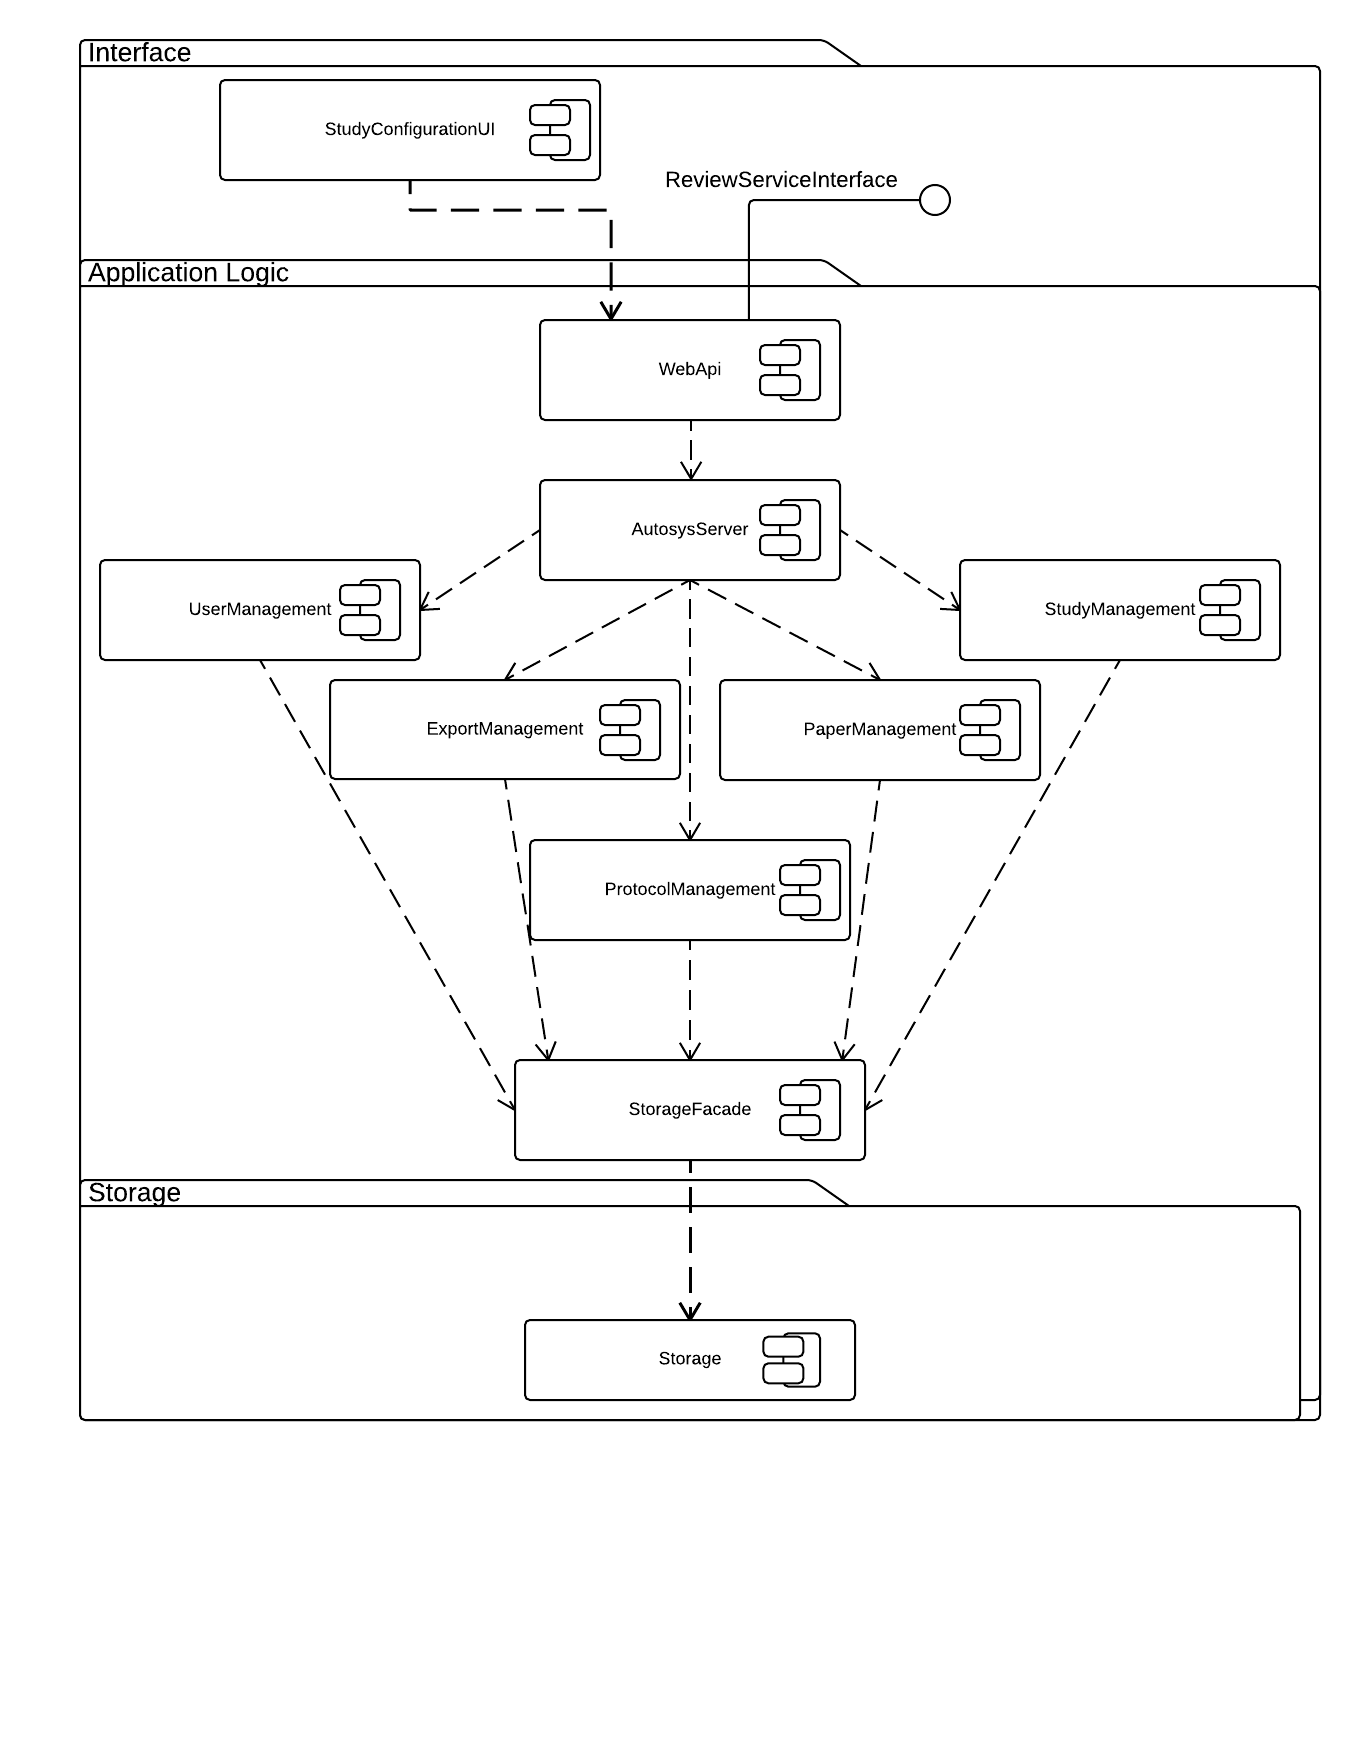
\includegraphics[width = \linewidth]{subsections/UMLComponentDiagramSubsystems}
	\caption{Autosys subsystem decomposition (UML Component Diagram, layers shown as UML packages)}
	\label{fig:Subsystem Decomposition, UML Component Diagram}
\end{figure}
The subsystems are identified from the functional requirements of the Autosys RAD document. A three-tier architectural style has been used for the decomposition of the system where a \textbf{StudyConfigurationClient} provides a front end for users to initiate all use cases related to setting up or configuring a \textbf{Study}. Also a \textbf{StudyReviewClient} will provide the front end for users to manage teams, and work with review tasks.
The \textbf{AutosysServer} will be managing access control, concurrency control, and delegates to nested subsystems for the application logic. The \textbf{UserManagement} component is holding the responsibility for handling all CRUD operations regarding teams and individual users. The processing of all Study related CRUD operations are carried out by the \textbf{StudyManagement} component. The  \textbf{StudyManagement} also manages Study Tasks, Study Criteria and Classifications, Study Phases and he other parts included in a study. The \textbf{PaperManagement} runs the filtering mechanisms on the research papers and does import/export of research papers according to the Study Criteria and Classifications.
The\textbf{ IStorage} interface is used for a Bridge Pattern to decouple the storage abstraction from the application logic so that the two can vary independently. At the bottom tier the \textbf{AutosysStorage} represents the subsystem for storing the user data, study data, and research papers.
	\input{subsection/PackageOverview}
	\input{subsection/PackageDependencies}
	\input{subsection/PackagePurpose}
\section{Class interfaces}
	\input{subsection/Classes} % Include class diagrams 
	\input{subsection/PublicInterfaces}
	\input{subsection/Dependencies}
	\input{subsection/Operations}
	\input{subsection/Attributes}
	\input{subsection/Exceptions}
\section{Design Decisions}
	\input{subsection/CodeStructure}
	\input{subsection/Solid}
	\input{subsection/Examples}
\section{Design Patterns}
	\input{subsection/BridgePatternBetweenLogicAndStorage}
	\input{subsection/RepositoryPatternInDatabase}
	\input{subsection/MappingBetweenLayers}
	\input{subsection/UIMVVMPattern}
	\input{subsection/Adapter pattern in WebApi}
	\input{subsection/Adapter pattern in ApplicationLogic}
\section{Discussion} % Relate used design decisions to SOLID principles

\end{document}